\section{Stabiliteitsberekening per ontwerp}
\label{sec:stab_ontwerpen}

Voor elk van de drie inrichtingsontwerpen is de dwarsscheepse stabiliteit
bepaald. De metacentrische hoogte $GM$ dient te voldoen aan het IMO-minimum
\cite[p.~44]{Barras2006}:

\begin{equation}
    GM = KB + BM - KG \geq 0{,}15\ \mathrm{m}
    \label{eq:GM_ontwerpen}
\end{equation}

De scheepsgeometrie en stabiliteitparameters voor de lege conditie
($KB_\mathrm{leeg} = 0{,}803$~m, $BM_\mathrm{leeg} = 1{,}384$~m,
$KG_\mathrm{leeg} = 1{,}30$~m) zijn voor alle ontwerpen gelijk aan de
waarden uit Hoofdstuk~\ref{chap:stabiliteit}. Alleen de ladingmassa
en het zwaartepunt van de lading verschillen per ontwerp.

% ----------------------------------------------------------
\subsection{Samenstelling en zwaartepuntschatting lading}
\label{sec:stab_samenstelling}

De drie ontwerpen onderscheiden zich in de verhouding zeezoutbatterijen en
LFP-modules. Een zeezoutcel ($18{,}7$~kg, $0{,}60 \times 0{,}39 \times
0{,}23$~m) is lichter dan een LFP-module ($40{,}0$~kg, $0{,}531 \times
0{,}206 \times 0{,}295$~m). Om het zwaartepunt van de lading zo laag
mogelijk te houden, worden de zwaardere LFP-modules altijd als onderste laag
geplaatst.

Het zwaartepunt van de lading $z_\mathrm{lad}$ is de hoogte boven de kiel.
Op basis van de scheepstekening \cite{JansjeTekening2026} bedraagt de
ruimbodem $\approx 0{,}30$~m boven kiel. De LFP-modules (hoogte $0{,}295$~m)
hebben daarmee een zwaartepunt op $0{,}30 + 0{,}148 \approx 0{,}45$~m boven
kiel. De zeezoutcellen worden daarboven gestapeld; het gemiddelde midden van
de stapel ligt op $0{,}30 + 1{,}00 = 1{,}30$~m boven kiel. Het gewogen
gemiddelde $z_\mathrm{lad}$ per ontwerp volgt uit:

\begin{equation}
    z_\mathrm{lad} =
    \frac{n_\mathrm{LFP} \cdot m_\mathrm{LFP} \cdot z_\mathrm{LFP}
        + n_z \cdot m_z \cdot z_z}
         {n_\mathrm{LFP} \cdot m_\mathrm{LFP} + n_z \cdot m_z}
    \label{eq:z_lad}
\end{equation}

\begin{table}[H]
\centering
\caption{Batterijsamenstelling en zwaartepuntschatting lading per ontwerp.
         Alle hoogten zijn gemeten boven de kiel \cite{JansjeTekening2026}.}
\label{tab:samenstelling}
\begin{tabular}{lcccccc}
\toprule
Ontwerp & $n_z$ & $n_\mathrm{LFP}$
        & $M_\mathrm{lad}$ [t]
        & $z_z$ [m] & $z_\mathrm{LFP}$ [m] & $z_\mathrm{lad}$ [m] \\
\midrule
1 -- zo duurzaam mogelijk & 91 & 12 & 2{,}18 & 1{,}30 & 0{,}45 & 1{,}24 \\
2 -- zo goedkoop mogelijk & 60 & 18 & 1{,}84 & 1{,}30 & 0{,}45 & 1{,}04 \\
3 -- hybride              & 70 & 14 & 1{,}87 & 1{,}30 & 0{,}45 & 1{,}14 \\
\bottomrule
\end{tabular}
\vspace{4pt}

\noindent\footnotesize
\textit{%
$n_z$: aantal zeezoutcellen ($m_z = 18{,}7$~kg);
$n_\mathrm{LFP}$: aantal LFP-modules ($m_\mathrm{LFP} = 40{,}0$~kg).
$z_z = 1{,}30$~m: zwaartepunt zeezoutcellen boven kiel
(ruimbodem $0{,}30$~m $+$ gemiddeld halve stapelhoogte $\approx 1{,}00$~m).
$z_\mathrm{LFP} = 0{,}45$~m: zwaartepunt LFP-modules boven kiel
(ruimbodem $0{,}30$~m $+$ halve modulehoogte $0{,}148$~m).
Ruimbodemhoogte afgeleid uit scheepstekening \cite{JansjeTekening2026}.}
\end{table}

% ----------------------------------------------------------
\subsection{Rekenmodel}
\label{sec:stab_rekenmodel}

De stabiliteitparameters in geladen conditie worden als volgt bepaald:

\begin{align}
    T_\mathrm{gel}  &= T_\mathrm{leeg} + \frac{M_\mathrm{lad}}{A_{WP}}
    \label{eq:T_gel} \\[4pt]
    KB_\mathrm{gel} &= 0{,}535 \times T_\mathrm{gel}
    \label{eq:KB_gel} \\[4pt]
    BM_\mathrm{gel} &= \frac{I_T}{\nabla_\mathrm{gel}}
                     = \frac{101{,}1}{\nabla_\mathrm{leeg} + M_\mathrm{lad}}
    \label{eq:BM_gel} \\[4pt]
    KG_\mathrm{gel} &= \frac{W \cdot KG_\mathrm{leeg}
                            + M_\mathrm{lad} \cdot z_\mathrm{lad}}
                            {W + M_\mathrm{lad}}
    \label{eq:KG_gel} \\[4pt]
    GM_\mathrm{gel} &= KB_\mathrm{gel} + BM_\mathrm{gel} - KG_\mathrm{gel}
    \label{eq:GM_gel}
\end{align}

met $A_{WP} = 77{,}0\ \mathrm{m^2}$, $\nabla_\mathrm{leeg} = 73{,}0\ \mathrm{m^3}$
en $W = 73{,}0\ \mathrm{t}$.

% ----------------------------------------------------------
\subsection{Ontwerp 1 -- zo duurzaam mogelijk}
\label{sec:stab_ontwerp1}

Ontwerp~1 bevat 91~zeezoutcellen en 12~LFP-modules
($M_1 = 2{,}18$~t, $z_\mathrm{lad,1} = 1{,}24$~m).

\begin{align}
    T_{\mathrm{gel},1}      &= 1{,}500 + \tfrac{2{,}18}{77{,}0}
                             = 1{,}528\ \mathrm{m}
                             \quad(\text{vrijboord} = 0{,}522\ \mathrm{m}) \\[4pt]
    \nabla_{\mathrm{gel},1} &= 73{,}0 + 2{,}18 = 75{,}2\ \mathrm{m^3} \\[4pt]
    KB_{\mathrm{gel},1}     &= 0{,}535 \times 1{,}528 = 0{,}817\ \mathrm{m} \\[4pt]
    BM_{\mathrm{gel},1}     &= \tfrac{101{,}1}{75{,}2} = 1{,}345\ \mathrm{m} \\[4pt]
    KG_{\mathrm{gel},1}     &= \frac{73{,}0 \times 1{,}30 + 2{,}18 \times 1{,}24}
                                    {75{,}2}
                             = \frac{94{,}90 + 2{,}70}{75{,}2}
                             = 1{,}298\ \mathrm{m} \\[6pt]
    \Aboxed{GM_{\mathrm{gel},1}} &\Aboxed{= 0{,}817 + 1{,}345 - 1{,}298
                             = 0{,}864\ \mathrm{m}}
\end{align}

% ----------------------------------------------------------
\subsection{Ontwerp 2 -- zo goedkoop mogelijk}
\label{sec:stab_ontwerp2}

Ontwerp~2 bevat 60~zeezoutcellen en 18~LFP-modules
($M_2 = 1{,}84$~t, $z_\mathrm{lad,2} = 1{,}04$~m). De relatief grote
fractie zware LFP-modules onderaan geeft het laagste ladingszwaartepunt
van de drie ontwerpen.

\begin{align}
    T_{\mathrm{gel},2}      &= 1{,}500 + \tfrac{1{,}84}{77{,}0}
                             = 1{,}524\ \mathrm{m}
                             \quad(\text{vrijboord} = 0{,}526\ \mathrm{m}) \\[4pt]
    \nabla_{\mathrm{gel},2} &= 73{,}0 + 1{,}84 = 74{,}8\ \mathrm{m^3} \\[4pt]
    KB_{\mathrm{gel},2}     &= 0{,}535 \times 1{,}524 = 0{,}815\ \mathrm{m} \\[4pt]
    BM_{\mathrm{gel},2}     &= \tfrac{101{,}1}{74{,}8} = 1{,}352\ \mathrm{m} \\[4pt]
    KG_{\mathrm{gel},2}     &= \frac{73{,}0 \times 1{,}30 + 1{,}84 \times 1{,}04}
                                    {74{,}8}
                             = \frac{94{,}90 + 1{,}91}{74{,}8}
                             = 1{,}294\ \mathrm{m} \\[6pt]
    \Aboxed{GM_{\mathrm{gel},2}} &\Aboxed{= 0{,}815 + 1{,}352 - 1{,}294
                             = 0{,}873\ \mathrm{m}}
\end{align}

% ----------------------------------------------------------
\subsection{Ontwerp 3 -- hybride}
\label{sec:stab_ontwerp3}

Ontwerp~3 bevat 70~zeezoutcellen en 14~LFP-modules
($M_3 = 1{,}87$~t, $z_\mathrm{lad,3} = 1{,}14$~m).

\begin{align}
    T_{\mathrm{gel},3}      &= 1{,}500 + \tfrac{1{,}87}{77{,}0}
                             = 1{,}524\ \mathrm{m}
                             \quad(\text{vrijboord} = 0{,}526\ \mathrm{m}) \\[4pt]
    \nabla_{\mathrm{gel},3} &= 73{,}0 + 1{,}87 = 74{,}9\ \mathrm{m^3} \\[4pt]
    KB_{\mathrm{gel},3}     &= 0{,}535 \times 1{,}524 = 0{,}815\ \mathrm{m} \\[4pt]
    BM_{\mathrm{gel},3}     &= \tfrac{101{,}1}{74{,}9} = 1{,}350\ \mathrm{m} \\[4pt]
    KG_{\mathrm{gel},3}     &= \frac{73{,}0 \times 1{,}30 + 1{,}87 \times 1{,}14}
                                    {74{,}9}
                             = \frac{94{,}90 + 2{,}13}{74{,}9}
                             = 1{,}294\ \mathrm{m} \\[6pt]
    \Aboxed{GM_{\mathrm{gel},3}} &\Aboxed{= 0{,}815 + 1{,}350 - 1{,}294
                             = 0{,}871\ \mathrm{m}}
\end{align}

% ----------------------------------------------------------
\subsection{Vergelijkingstabel}
\label{sec:stab_vergelijk}

\begin{table}[H]
\centering
\caption{Stabiliteitscomponenten per ontwerp -- geladen conditie}
\label{tab:stab_vergelijk}
\begin{tabular}{lrrrrl}
\toprule
Grootheid & Leeg & Ontwerp 1 & Ontwerp 2 & Ontwerp 3 & Eenheid \\
\midrule
\multicolumn{6}{l}{\textit{Lading}} \\[2pt]
Zeezoutcellen $n_z$          &  --     &  91     &  60     &  70     & --    \\
LFP-modules $n_\mathrm{LFP}$ &  --     &  12     &  18     &  14     & --    \\
Ladingmassa $M_\mathrm{lad}$ &  --     & 2{,}18  & 1{,}84  & 1{,}87  & t     \\
\midrule
\multicolumn{6}{l}{\textit{Drijfvermogen}} \\[2pt]
Diepgang $T$                 & 1{,}500 & 1{,}528 & 1{,}524 & 1{,}524 & m     \\
Vrijboord                    & 0{,}550 & 0{,}522 & 0{,}526 & 0{,}526 & m     \\
$\nabla$                     & 73{,}0  & 75{,}2  & 74{,}8  & 74{,}9  & m$^3$ \\
\midrule
\multicolumn{6}{l}{\textit{Stabiliteitscomponenten}} \\[2pt]
$KB$                         & 0{,}803 & 0{,}817 & 0{,}815 & 0{,}815 & m \\
$BM$                         & 1{,}384 & 1{,}345 & 1{,}352 & 1{,}350 & m \\
$KG$                         & 1{,}300 & 1{,}298 & 1{,}294 & 1{,}294 & m \\
\midrule
\rowcolor{green!15}
$GM$ & \textbf{0{,}887} & \textbf{0{,}864}
     & \textbf{0{,}873} & \textbf{0{,}871} & m \\
\midrule
\multicolumn{6}{l}{\textit{Toetsing}} \\[2pt]
IMO-min.\ $GM \geq 0{,}15$~m \cite[p.~44]{Barras2006}
  & \checkmark & \checkmark & \checkmark & \checkmark & -- \\
Vrijboord $\geq 0{,}20$~m
  & \checkmark & \checkmark & \checkmark & \checkmark & -- \\
\bottomrule
\end{tabular}
\end{table}

% ----------------------------------------------------------
\subsection{Grafische vergelijking}
\label{sec:stab_grafiek}

\begin{figure}[H]
\centering
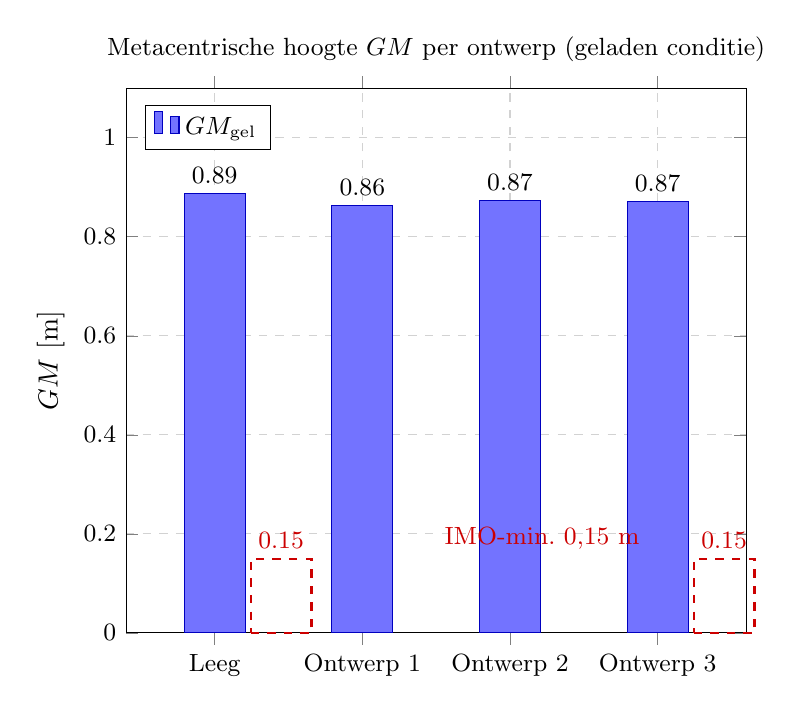
\begin{tikzpicture}
\begin{axis}[
    ybar,
    bar width        = 22pt,
    width            = 0.78\textwidth,
    height           = 8.5cm,
    enlarge x limits = 0.20,
    symbolic x coords= {Leeg,{Ontwerp 1},{Ontwerp 2},{Ontwerp 3}},
    xtick            = data,
    xticklabel style = {font=\small},
    ylabel           = {$GM$ [m]},
    ymin             = 0,
    ymax             = 1.10,
    % Nette ytick-waarden zonder overlap met de stippellijn-labels
    ytick            = {0, 0.2, 0.4, 0.6, 0.8, 1.0},
    yticklabel style = {/pgf/number format/fixed,
                        /pgf/number format/precision=1,
                        font=\small},
    nodes near coords,
    nodes near coords align = {above},
    every node near coord/.append style = {font=\small},
    grid             = major,
    grid style       = {dashed, gray!35},
    % Legenda linksbovenin zodat die niet overlapt met balken
    legend style     = {at={(0.03,0.97)}, anchor=north west, font=\small},
    title            = {Metacentrische hoogte $GM$ per ontwerp (geladen conditie)},
    title style      = {font=\small},
    clip             = false,   % zodat node buiten plotgebied kan staan
]

%% Blauwe balken
\addplot[fill=blue!55, draw=blue!75!black]
    coordinates {
        (Leeg,        0.887)
        ({Ontwerp 1}, 0.864)
        ({Ontwerp 2}, 0.873)
        ({Ontwerp 3}, 0.871)
    };
\addlegendentry{$GM_\mathrm{gel}$}

%% IMO-minimum -- één doorlopende lijn van links naar rechts
\addplot[
    thick, red!80!black, dashed, forget plot
] coordinates {(Leeg, 0.15) ({Ontwerp 3}, 0.15)};

%% IMO-label: boven de lijn, vlak bij de rechteras, buiten de laatste balk
\node[
    red!80!black, font=\small, anchor=south east
] at (axis cs:{Ontwerp 3}, 0.15) {IMO-min.\ $0{,}15$~m \quad};

\end{axis}
\end{tikzpicture}
\caption{$GM$ in geladen conditie voor de lege toestand en de drie
         batterijontwerpen. De gestippelde rode lijn geeft het IMO-minimum
         van $0{,}15$~m weer \cite[p.~44]{Barras2006}. Alle ontwerpen
         voldoen ruimschoots. Ruimbodemhoogte gebaseerd op scheepstekening
         \cite{JansjeTekening2026}.}
\label{fig:GM_vergelijk}
\end{figure}

% ----------------------------------------------------------
\subsection{Conclusie}
\label{sec:stab_conclusie_ontwerpen}

Alle drie de ontwerpen voldoen ruimschoots aan het IMO-minimum van
$0{,}15$~m. De metacentrische hoogte in geladen conditie ligt voor elk
ontwerp in het bereik $0{,}864$--$0{,}873$~m. Het onderlinge verschil
tussen de ontwerpen bedraagt maximaal $0{,}009$~m en is daarmee
verwaarloosbaar. De stabiliteit vormt voor geen van de ontwerpen een
beperkende factor bij de ontwerpselectie.


\subsection{Ontwerpkeuze?}

Nu de keuze is gemaakt voor ontwerp 1 moet worden onderzocht of het systeem voldoet aan de eisen. In het systeem zijn 91 zeezoutbatterijen en 12 LFP-batterijen. Echter is de capaciteit die met deze hoeveelheid batterijen bereikt wordt meer dan de eerder gestelde randvoorwaarde van 108.15 kWh \ref{}, namelijk 113.28 \ref{}. Daarom kan er in theorie worden bespaard op de hoeveelheid zeezoutbatterijen. Deze hebben een lagere capaciteit dan de LFP-batterij (0.48 kWh tegenover 5.8 kWh) waardoor enkel met minder zeezoutbatterijen nog voldaan kan worden aan de randvoorwaarde. Door negen zeezoutbatterijen minder mee te nemen is de capaciteit 108.96 kWh, hiermee wordt nog steeds voldaan aan de randvoorwaarde. 

\noindent Een schip dat vaart op elektrische batterijen kan gebruik maken van verschillende voltages, er zijn meerdere opties. Een laag voltage betekent dat de stroomsterkte door de kabels hoog is. Dit brengt bepaalde veiligheidsrisico's en complicaties met zich mee maar is wel erg efficiënt. Aan de andere kant betekent een hoog voltage dat de stroomsterkte lager is en de gebruiksgemak veiligheidrisico's hoger zijn. Zoals eerder benoemd zijn er 82 zeezoutbatterijen en 12 LFP-batterijen nodig. Beide batterijen leveren standaard 24 V \ref{}\ref{}, om een voltage van 48 V te bereiken moeten paren worden gemaakt van 


\begin{table}[h!]
\centering
\caption{Vergelijking van Batterijconfiguraties voor Het Jansje (Basis: 12 LFP en 90 Zeezout)}
\label{tab:batterij_vergelijking_compleet}
\begin{tabular}{|l||l|c|c|c|c|}
\hline
\textbf{Systeemspanning} & \textbf{Batterijtype} & \textbf{Schakeling} & \textbf{Max. Vermogen} & \textbf{Stroomsterkte} & \textbf{Totale Opslag} \\ 
 & & \textbf{(Serie / Parallel)} &  & & \\ \hline\hline

 & LFP  & $1\text{S} \times 12\text{P}$ & 70.68 kW & & 69.60 kWh \\ \cline{2-4} \cline{6-6}
\textbf{24 V} & Zeezout & $1\text{S} \times 90\text{P}$ & 16.83 kW & 916.7 A & 43.20 kWh \\ \cline{2-4} \cline{6-6}
 & \textbf{Totaal} & \textbf{--} & \textbf{87.51 kW} & & \textbf{112.80 kWh} \\ \hline\hline

 & LFP  & $2\text{S} \times 6\text{P}$ & 35.34 kW & & 69.60 kWh \\ \cline{2-4} \cline{6-6}
\textbf{48 V} & Zeezout & $2\text{S} \times 41\text{P}$ & 7.67 kW & 458.3 A & 39.36 kWh \\ \cline{2-4} \cline{6-6}
 & \textbf{Totaal} & \textbf{--} & \textbf{43.01 kW} & & \textbf{108.96 kWh} \\ \hline\hline

 & LFP  & $3\text{S} \times 4\text{P}$ & 23.56 kW & & 69.60 kWh \\ \cline{2-4} \cline{6-6}
\textbf{72 V} & Zeezout & $3\text{S} \times 30\text{P}$ & 5.61 kW & 305.6 A & 43.20 kWh \\ \cline{2-4} \cline{6-6}
 & \textbf{Totaal} & \textbf{--} & \textbf{29.17 kW} & & \textbf{112.80 kWh} \\ \hline\hline

 & LFP & $4\text{S} \times 3\text{P}$ & 17.67 kW & & 69.60 kWh \\ \cline{2-4} \cline{6-6}
\textbf{96 V} & Zeezout & $4\text{S} \times 20\text{P}$ & 3.74 kW & 229.2 A & 38.40 kWh \\ \cline{2-4} \cline{6-6}
 & \textbf{Totaal} & \textbf{--} & \textcolor{red}{21.41 kW} & & \textcolor{red}{108.00 kWh} \\ \hline\hline

 & LFP & $5\text{S} \times 2\text{P}$ & 11.78 kW & & 58.00 kWh \\ \cline{2-4} \cline{6-6}
\textbf{120 V} & Zeezout & $5\text{S} \times 18\text{P}$ & 3.37 kW & 183.3 A & 43.20 kWh \\ \cline{2-4} \cline{6-6}
 & \textbf{Totaal} & \textbf{--} & \textcolor{red}{15.15 kW} & & \textcolor{red}{101.20 kWh} \\ \hline\hline
\end{tabular}
\end{table}

Bij de oplossing met een voltage van 48 V worden maar 82 zeezoutbatterijen gebruikt, dit is precies de minimale hoeveelheid en dus kan de rest zo worden geschakeld dat deze dienen als reservevoorziening.
Deze overige negen kunnen worden gebruikt als reserve energievoorziening om te voldoen aan de veiligheidseis \ref{}. 







\chapter{Aandrijfsysteemkeuze}

\noindent Nu het energieopslagstysteem is bepaald, kan onderzocht worden wat de meeste geschikte aandrijving zal zijn. Dit is tevens deelvraag 3:
\begin{quote}
    \textit{\textbf{Welk aandrijfsysteem is het meest geschikt voor transportschip Jansje, rekening houdend met
het gekozen energieopslagsysteem en het programma van eisen?}}
\end{quote}
\noindent Het gekozen energieopslagsysteem is een combinatie van zeezoutbatterijen en LFP batterijen. Dit zorgt er in ieder geval voor dat de huidige dieselmotor zal moeten worden vervangen door een elektromotor, in het geval dat keuze op een bio-brandstof zou vallen zou deze nog kunnen worden omgebouwd en hergebruikt maar in deze configuratie is dat geen optie. In dit hoofdstuk zullen randvoorwaarden worden opgesteld waaraan de nieuwe elektromotor zal moeten voldoen. Vervolgens zullen verschillende elektromotoren worden vergeleken en zal de best mogelijke optie worden gekozen.

\subsection{Randvoorwaarden}
\begin{enumerate}
    \item Het minimale benodigde vermogen wat de elektromotor aan zal moeten kunnen, bedraagt 22 kW \ref{}.
    \item De schroef draait in het huidige systeem op 600 RPM \cite{mail arnold}, dit betekent dat de nieuwe motor op hetzelfde toerenaantal zal moeten draaien of dat er een overbrenging nodig is. 
    \item Bij een toerental van 600 RPM is een koppel van 350 Nm nodig zoals berekend in de bijlage \ref{eq:koppelberekening}
    \item Uit metingen die plaats hebben gevonden op het schip blijkt dat de beschikbare ruimte voor het aandrijfsysteem (lxbxh) 1.4 x 0.7 x 1.0 m is.     
    \item Het voltage van de elektromotor bedraagt 48 V \ref{}.
    \item Vanwege het feit dat het energieopslagsysteem van het schip een direct stroom levert (DC) \cite{} is het rekening houdend met de kosten handig om een DC- motor aan te schaffen. Echter is het met een conversiesysteem wel mogelijk om gebruik te maken van een AC- motor dus hoeft deze optie niet uitgesloten te worden. 
\end{enumerate}



\noindent 

\section{}
Als een motor aan de bovenstaande eisen voldoet, kan deze worden toegepast in Jansje. Er zijn veel verschillende motoren op de markt met geschikte eigenschappen die goed bij Jansje zouden kunnen passen. Daarom is er één voorbeeldmotor gekozen om onder andere de prijs te kunnen bepalen. Een andere motor die aan dezelfde eisen voldoet, zou in principe ook geschikt kunnen zijn.


\subsection{Voorbeeld motor}
Als voorbeeldmotor is gekozen voor de GM22.5 Elektromotor van Green Marine. Deze motor is geselecteerd omdat Green Marine een Nederlands bedrijf is en de motor daardoor goed aansluit bij de Nederlandse markt. De prijs kan daarom worden gebruikt als realistische indicatie voor vergelijkbare motoren die mogelijk geschikt zijn voor Jansje. Omdat de motor een nominaal toerental van 1200 rpm heeft en het gewenste schroefastoerental 600 rpm is, is een 2:1 reductieoverbrenging nodig.

\begin{table}[h]
    \centering
    \caption{Belangrijkste specificaties van de GM22.5 elektromotor}
    \label{tab:gm22-5-motor}
    \begin{tabular}{ll}
        \hline
        \textbf{Eigenschap} & \textbf{Waarde\cite{greenmarine_gm225_datasheet}} \\
        \hline
        Model & GM22.5 Elektromotor \\
        Motortype & 3-fase PMSM \\
        Prijs & Nog te bepalen via mailcontact \\
        Vermogen & 22.5 kW \\
        Accuspanning & 40--65 V, 48 V nominaal \\
        Maximaal koppel & 180 Nm \\
        Nominaal toerental & 1200 rpm \\
        IP-klasse & IP68 \\
        Gewicht motor & ca. 65 kg \\
        Minimale kabeldikte & 120 mm$^2$ \\
        \hline
    \end{tabular}
\end{table}
